\documentclass[conference]{IEEEtran}

\usepackage{cite}
\usepackage{amsmath,amssymb,amsfonts}
\usepackage{graphicx}
\usepackage{textcomp}
\usepackage{xcolor}
\usepackage{booktabs}
\usepackage{array}
\usepackage{tikz}
\usepackage{url}
\usetikzlibrary{arrows.meta,positioning}

\def\BibTeX{{\rm B\kern-.05em{\sc i\kern-.025em b}\kern-.08em
    T\kern-.1667em\lower.7ex\hbox{E}\kern-.125emX}}

\newcommand{\THD}{\mathrm{THD}}
\newcommand{\TDD}{\mathrm{TDD}}

\begin{document}

\title{Finite-Control-Set Model Predictive Control of Shunt Active Harmonic Filters for Industrial Applications}

\author{\IEEEauthorblockN{Anna May A. Rapi\~{n}an}
\IEEEauthorblockA{\textit{Ateneo de Naga University}\\
Naga City 4400, Philippines\\
arapinan@gbox.adnu.edu.ph}}

\maketitle

\begin{abstract}
Industrial power systems increasingly rely on nonlinear loads, such as variable-frequency drives, rectifier front ends, and converter-interfaced distributed generation, that improve energy efficiency but severely degrade power quality. These loads draw non-sinusoidal currents that lead to voltage distortion, transformer heating, capacitor-bank resonance, and protection misoperation. This study develops active harmonic filtering as a control-system problem rather than as an isolated power-electronics accessory. Establishing the harmonic-current model and performance quantities defined in IEEE Std 519-2022 and IEEE Std 1459-2025, the study derives the compensating-current objective for active harmonic mitigation. Reference-generation methods are systematically compared through their control assumptions, spanning instantaneous power theory to advanced finite-control-set model predictive control (FCS-MPC). By evaluating shunt, series, hybrid, and unified power quality conditioner topologies against parameters of rating, sensing, and protection, the study concludes that the shunt active filter provides the most direct solution for industrial current-harmonic problems. Series and hybrid structures remain justified primarily when feeder-level harmonic isolation or passive-filter interactions dictate the design.
\end{abstract}

\begin{IEEEkeywords}
Finite-control-set, harmonic compensation, nonlinear loads, power quality, reference generation, total harmonic distortion.
\end{IEEEkeywords}

\section{Introduction}
The growth of power-electronic loads has changed the nature of facility power-quality design. A conventional sinusoidal load draws current at the fundamental frequency; an industrial nonlinear load draws current in pulses, and those pulses can be decomposed into harmonic components. In a three-phase facility, six-pulse rectifiers characteristically generate $6n\pm1$ current harmonics, while single-phase diode-capacitor supplies produce narrow current peaks and four-wire systems can carry substantial triplen and neutral current. The result is not merely a distorted waveform on an oscilloscope. It is extra rms current, additional heating, possible resonance with capacitor banks, nuisance operation of protective equipment, and voltage distortion seen by other loads on the same bus.

Passive tuned filters remain useful when harmonic orders, source impedance, and loading are known with confidence. Their limitation is that an industrial bus is rarely fixed: drives start and stop, process loading changes, capacitor banks switch, and standby generators can change the available short-circuit strength. Active harmonic filters (AHFs), also called active power filters (APFs), address this changing condition by measuring the waveform, calculating the undesired current or voltage component, and injecting a compensating waveform in real time. The idea grew from instantaneous reactive power compensation proposed by Akagi, Kanazawa, and Nabae \cite{Akagi1984}, evolved into practical active and hybrid filters \cite{Peng1990,Akagi1996}, and became a mature power-conditioning technology reviewed extensively in the literature \cite{Singh1999,ElHabrouk2000,Akagi2005}.

The study's direction is therefore design oriented. It asks what a professional engineer should check before specifying an AHF: the standard to be satisfied, the harmonic quantity to be reduced, the control method that generates the reference, the topology that injects the compensation, and the practical limits imposed by rating, sensing, and protection. This organization avoids treating control methods as isolated inventions. Instead, each method is discussed according to how it helps the filter satisfy a measurable power-quality target at the point of common coupling (PCC).

\section{Harmonic Problem and Performance Criteria}
\subsection{Load-Current Model}
For a steady periodic distorted current, the load current can be expressed as a fundamental component plus harmonic components:
\begin{equation}
i_L(t)=I_1\sin(\omega t-\phi_1)+\sum_{h=2}^{H} I_h\sin(h\omega t-\phi_h).
\label{eq:fourier}
\end{equation}
In \eqref{eq:fourier}, $i_L(t)$ is the instantaneous load current, $I_1$ and $\phi_1$ are the magnitude and phase angle of the fundamental component, and $I_h$ and $\phi_h$ describe the $h$th harmonic up to the highest order $H$ considered in the measurement. The equation is important because the AHF does not need to guess the load type; it only needs to identify which terms in the measured current should remain in the source current and which terms should be supplied locally by the filter. In other words, the harmonic model defines the control objective.

The usual current total harmonic distortion is
\begin{equation}
\THD_I=\frac{\sqrt{\sum_{h=2}^{H} I_h^2}}{I_1}\times100\%.
\label{eq:thd}
\end{equation}
Equation \eqref{eq:thd} compares all rms harmonic current to the rms fundamental current. It is useful for judging waveform shape, but it can overstate a facility concern at light load because $I_1$ becomes small. For compliance-oriented industrial studies, total demand distortion is often the more relevant current quantity:
\begin{equation}
\TDD=\frac{\sqrt{\sum_{h=2}^{H} I_h^2}}{I_L}\times100\%,
\label{eq:tdd}
\end{equation}
where $I_L$ is the maximum demand load current at the PCC. Equation \eqref{eq:tdd} normalizes harmonic current to the facility demand current, so it better reflects the burden imposed on the utility interface. IEEE Std 519-2022 uses PCC-based harmonic current and voltage distortion limits, with current limits related to the ratio of available short-circuit current to maximum demand current \cite{IEEE5192022}. IEEE Std 1459-2025 complements this by defining power quantities under sinusoidal, nonsinusoidal, balanced, and unbalanced conditions, which matters because poor power factor may be caused by displacement, distortion, unbalance, or a combination of the three \cite{IEEE14592025}.

\subsection{Engineering Interpretation}
The practical implication of \eqref{eq:fourier}--\eqref{eq:tdd} is that the AHF rating should be tied to measured harmonic current and the required residual distortion at the PCC. A filter specified only by a nominal ampere value can be misleading: a 100-A unit may be adequate for a drive bus with modest 5th and 7th harmonic current but inadequate for a four-wire commercial panel with high triplen neutral current. The engineering target should therefore include measured harmonic spectrum, maximum demand current, voltage distortion background, load diversity, and the operating condition under which compliance is required.

\section{Active Harmonic Cancellation as a Control Problem}
The shunt AHF is the most common industrial form because most facility harmonic issues are load-current issues. At the bus where the filter is connected, Kirchhoff's current law gives
\begin{equation}
i_s(t)=i_L(t)+i_c(t),
\label{eq:kcl}
\end{equation}
where $i_s(t)$ is the source current, $i_L(t)$ is the nonlinear load current, and $i_c(t)$ is the current injected by the filter. Equation \eqref{eq:kcl} makes the cancellation principle explicit: the source current is not cleaned by destroying harmonic current, but by making the filter supply the nonfundamental portion locally. If the desired source current is a balanced sinusoid $i_s^{*}(t)$, then the reference compensating current is
\begin{equation}
i_c^{*}(t)=i_s^{*}(t)-i_L(t).
\label{eq:reference}
\end{equation}
Equation \eqref{eq:reference} is the central control law for a shunt filter. Under ideal current-harmonic compensation, $i_c^{*}$ is equal in magnitude and opposite in phase to the harmonic part of the load current. If reactive-power compensation is also required, $i_s^{*}$ is selected in phase with the fundamental positive-sequence voltage. If load balancing is required, negative- and zero-sequence components are also assigned to the filter.

\begin{figure}[!t]
\centering
\resizebox{\columnwidth}{!}{%
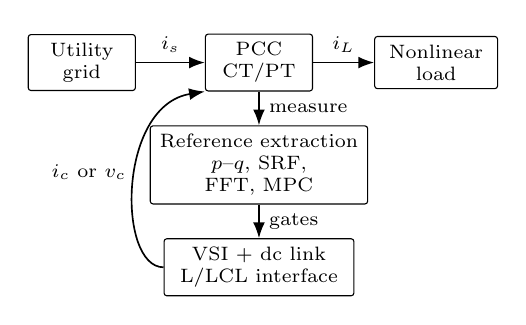
\begin{tikzpicture}[
    font=\scriptsize,
    >=Latex,
    block/.style={draw, rounded corners=1pt, align=center, minimum height=0.58cm, inner sep=3pt},
    line/.style={-Latex, semithick}
]
\node[block, text width=1.15cm] (grid) at (0,0) {Utility\\grid};
\node[block, text width=1.15cm] (pcc) at (2.25,0) {PCC\\CT/PT};
\node[block, text width=1.35cm] (load) at (4.50,0) {Nonlinear\\load};
\node[block, text width=2.55cm] (ctrl) at (2.25,-1.30) {Reference extraction\\$p$--$q$, SRF, FFT, MPC};
\node[block, text width=2.20cm] (vsi) at (2.25,-2.60) {VSI + dc link\\L/LCL interface};
\draw[line] (grid) -- node[above] {$i_s$} (pcc);
\draw[line] (pcc) -- node[above] {$i_L$} (load);
\draw[line] (pcc.south) -- node[right] {measure} (ctrl.north);
\draw[line] (ctrl.south) -- node[right] {gates} (vsi.north);
\draw[line] (vsi.west) .. controls (0.45,-2.60) and (0.45,-0.55) ..
    node[left,pos=0.55] {$i_c$ or $v_c$} (pcc.south west);
\end{tikzpicture}%
}
\caption{Active harmonic filter control architecture. The controller measures PCC and load quantities, extracts the compensating reference, and commands a converter to inject current for shunt filtering or voltage for series filtering.}
\label{fig:architecture}
\end{figure}

Fig.~\ref{fig:architecture} frames the AHF as a closed-loop control system. The plant is the converter, dc link, and coupling reactor or LCL interface. The controller has three jobs. First, it estimates the harmonic, reactive, unbalanced, or voltage-disturbance component to be compensated. Second, it regulates the dc link so converter losses are supplied without injecting unwanted real power. Third, it tracks the reference fast enough that harmonic cancellation remains accurate during load changes. Green and Marks classify these control functions as reference generation, current or voltage regulation, and energy-storage control \cite{Green2005}; more recent reviews show that the same structure remains the basis for present shunt APF designs \cite{Popescu2024}.

\section{Reference Extraction and Tracking}
\subsection{Instantaneous Power Theory}
Instantaneous power theory transforms three-phase quantities to stationary $\alpha$--$\beta$ axes and computes instantaneous real and imaginary power:
\begin{equation}
\begin{bmatrix}p\\q\end{bmatrix} =
\begin{bmatrix}v_{\alpha} & v_{\beta}\\ -v_{\beta} & v_{\alpha}\end{bmatrix}
\begin{bmatrix}i_{\alpha}\\i_{\beta}\end{bmatrix}.
\label{eq:pq}
\end{equation}
In \eqref{eq:pq}, $p$ is the instantaneous real power associated with energy transfer, and $q$ represents the instantaneous imaginary power in the $\alpha$--$\beta$ plane. The method separates average and oscillating components of $p$ and $q$; the oscillating components are then mapped back into current references for the filter. This theory is historically central to APF development \cite{Akagi1984,AkagiBook2007}. Its strength is fast time-domain response without waiting for one full fundamental cycle. Its limitation is that nonideal supply voltage changes the meaning of ``ideal'' compensation. Herrera, Salmeron, and Kim experimentally showed that different instantaneous-power formulations can produce different results under distorted or unbalanced source voltage \cite{Herrera2008}. Thus, the designer must state the target explicitly: unity power factor, sinusoidal source current, load balancing, or a prioritized combination.

\subsection{Synchronous Reference Frame Control}
The synchronous reference frame (SRF) method rotates measured currents into a $dq$ frame locked to the positive-sequence fundamental voltage. Fundamental active current becomes a dc quantity, while harmonics appear as ripple. Low-pass filtering can then separate the desired fundamental active component from harmonic and reactive components. SRF control is attractive because it works naturally with PI regulators, but it depends on phase-locked-loop quality and filter delay. Four-wire systems require additional care because neutral and zero-sequence currents must be compensated through a split dc link or a four-leg inverter. Aredes, Hafner, and Heumann treated three-phase four-wire shunt filter strategies \cite{Aredes1997}, while Montero, Cadaval, and Gonzalez compared control objectives for these systems under nonideal conditions \cite{Montero2007}.

\subsection{Selective, Adaptive, and Neural Detection}
Many plants do not need every harmonic cancelled with equal priority. Selective harmonic compensation targets the dominant orders, commonly the 5th, 7th, 11th, and 13th for six-pulse rectifier loads. This reduces converter burden and avoids asking the filter to chase noise or insignificant high-order components. Mattavelli's closed-loop selective compensation work shows how individual harmonic references can be regulated without treating the load current as one broadband error signal \cite{Mattavelli2001}. Detection remains critical: Asiminoaei, Blaabjerg, and Hansen showed that extraction method, selectivity, and delay largely determine the filter's final performance \cite{Asiminoaei2007}.

Adaptive and data-assisted methods extend selective compensation to loads whose spectra change with time. Pereira \textit{et al.} used adaptive notch filters with least-mean-square and recursive-least-square updating for shunt APFs, including DSP implementation \cite{Pereira2011}. Cirrincione, Pucci, and Vitale demonstrated adaptive neural filtering in a distributed-generation unit with shunt APF capability \cite{Cirrincione2008}. These methods are promising because they can adjust to changing loads, but their convergence, stability margins, and behavior outside the training or tuning envelope must be verified before deployment in critical industrial service.

\subsection{Current Control and Predictive Control}
Once the reference is generated, the converter must track it. Hysteresis control has fast response but variable switching frequency. Fixed-frequency PWM with PI or proportional-resonant controllers is easier to filter and coordinate with electromagnetic-interference requirements but can suffer from sampling and modulation delay. Deadbeat control improves speed but is sensitive to parameter error. Buso, Malesani, and Mattavelli compared these current-control methods and showed that the best choice depends on the required dynamic response, switching constraints, and implementation accuracy \cite{Buso1998}.

Finite-control-set model predictive control (FCS-MPC) evaluates converter switching states directly. A simplified one-step cost function is
\begin{equation}
u^{*}=\arg\min_{u_j}\left\|i_c^{*}(k+1)-\hat{i}_c(k+1,u_j)\right\|^2+\lambda_s\Delta s_j.
\label{eq:mpc}
\end{equation}
In \eqref{eq:mpc}, $u_j$ is a candidate switching state, $\hat{i}_c(k+1,u_j)$ is the predicted compensating current at the next sample if that state is applied, $i_c^{*}(k+1)$ is the desired next-sample reference, $\Delta s_j$ represents switching changes, and $\lambda_s$ weights switching effort against current error. The equation is rigorous because it makes the tradeoff visible: a controller can reduce current error by switching more often, but switching loss and electromagnetic noise must also be considered. Rodriguez \textit{et al.} and Vazquez \textit{et al.} identify this ability to handle multivariable constraints as a major strength of MPC in power electronics \cite{Rodriguez2013,Vazquez2014}. Guzman \textit{et al.} applied FCS-MPC with Kalman-filter estimation to a three-phase shunt APF, illustrating how predictive control can improve behavior under noisy measurements \cite{Guzman2017}.

\section{Topology and Hardware Selection}
\begin{table*}[!t]
\caption{Engineering Comparison of Active Harmonic Filter Topologies}
\label{tab:topologies}
\centering
\footnotesize
\setlength{\tabcolsep}{3pt}
\begin{tabular}{@{}p{0.13\textwidth}p{0.18\textwidth}p{0.17\textwidth}p{0.25\textwidth}p{0.15\textwidth}@{}}
\toprule
\textbf{Topology} & \textbf{Primary Disturbance} & \textbf{Injected Quantity} & \textbf{Best-Fit Application} & \textbf{Main Caution} \\
\midrule
Shunt active filter & Load current harmonics, reactive current, unbalance, neutral current & Compensating current in parallel with load & Variable-speed-drive buses, rectifier groups, commercial and industrial low-voltage switchboards & Rating must cover harmonic current and dynamic load change \\
Series active filter & Source voltage harmonics, voltage sag/swell, harmonic isolation & Compensating voltage in series with feeder & Sensitive loads exposed to distorted upstream voltage or weak feeder conditions & Must carry load current and satisfy insulation/protection requirements \\
Hybrid active-passive filter & Dominant fixed harmonics plus residual or resonance damping & Small active voltage/current plus passive branch current & Medium-voltage or high-power rectifier systems where full active rating is costly & Passive branch tuning and detuning must be studied over system changes \\
Unified power quality conditioner & Simultaneous current and voltage quality problems & Shunt current and series voltage with shared dc link & Critical process loads needing current cleanup and voltage conditioning & Highest control, protection, and commissioning complexity \\
\bottomrule
\end{tabular}
\end{table*}

Table~\ref{tab:topologies} connects topology choice to the disturbance being corrected. A shunt active filter is the default solution for current harmonics because it injects current at the bus and does not continuously carry the full load current. Its rating is usually determined by harmonic current and dynamic margin, not by total load current. In three-phase four-wire systems, the converter must also provide a neutral-current path if triplen harmonics are significant \cite{Aredes1997,Montero2007}.

A series active filter is a voltage-quality device. It injects voltage in series with the feeder to block source-voltage harmonics or isolate downstream nonlinear behavior from the upstream network. A pure series AHF must be protected carefully because it is inserted into the power path. Hybrid filters reduce active-converter rating by letting passive branches handle predictable harmonic orders while the active part damps resonance or corrects residual distortion. Peng, Akagi, and Nabae demonstrated the value of combining passive shunt filtering with series active compensation \cite{Peng1990}. A unified power quality conditioner integrates shunt and series converters through a common dc link, enabling both current and voltage conditioning, but with greater control and protection complexity \cite{Fujita1998}.

The converter hardware has also advanced. Multilevel converter families reduce device voltage stress and output ripple, making them attractive for medium-voltage and high-power AHFs; however, their capacitor balancing and fault modes must be controlled deliberately \cite{Franquelo2008}. Wide-bandgap silicon carbide and gallium nitride devices can increase switching frequency and reduce filter size, but they also raise electromagnetic-interference, insulation, and gate-drive layout requirements \cite{Millan2014}. These technologies improve the implementation of \eqref{eq:reference} and \eqref{eq:mpc}; they do not remove the need for a correctly defined compensation objective.

\section{Engineering Design Procedure}
\subsection{Rating and Placement}
A professional AHF specification should begin with measured or simulated harmonic data at the proposed installation point. The minimum data set includes voltage distortion, current spectrum, maximum demand current, load profile, transformer impedance, capacitor-bank status, generator operation, and existing filter equipment. Installing one filter at the service entrance may satisfy PCC compliance, while distributed filters near major nonlinear loads can reduce internal feeder heating and local voltage distortion. The correct placement depends on system impedance and the objective: utility compliance, internal power quality, equipment protection, or all three.

\subsection{Sensing, Stability, and Commissioning}
The control law in \eqref{eq:kcl} is only as reliable as the measurements used to implement it. Current-transformer polarity errors, incorrect CT ratio settings, noisy voltage sensing, or confusion between source and load current can make the filter reinforce harmonics instead of cancelling them. Commissioning should therefore include baseline measurements, verification of sensor orientation, staged load tests, dc-link ripple checks, thermal scans, and confirmation of protection selectivity. If the plant has automatic capacitor switching, the AHF should be tested through switching events because the network resonance and harmonic impedance can change abruptly.

\subsection{Recommended Selection Logic}
For a low-voltage motor-control center dominated by variable-frequency drives, a shunt AHF with SRF or selective harmonic compensation is typically the most practical solution. For a weak feeder where upstream voltage distortion affects sensitive equipment, a series or UPQC arrangement should be considered. For medium-voltage rectifier systems or large fixed harmonic sources, a hybrid active-passive solution may achieve the required $\TDD$ with lower active kVA, provided detuning and resonance are studied. Where the load spectrum varies rapidly, adaptive detection or FCS-MPC can improve response, but it should be justified by measured dynamics rather than selected only because it is newer.

\section{Conclusion}
Active harmonic filtering is best understood as a feedback-control application in power quality. The harmonic model in \eqref{eq:fourier}, the distortion metrics in \eqref{eq:thd} and \eqref{eq:tdd}, and the compensation law in \eqref{eq:reference} show that the filter's job is to make the source current match a defined target, not simply to ``remove harmonics'' in a vague sense. Instantaneous power theory and SRF control provide mature time-domain reference generation; selective, adaptive, neural, and predictive methods improve performance when spectra vary or constraints must be handled explicitly.

For most industrial current-harmonic cases, the shunt AHF remains the most direct and maintainable choice. Series filters, hybrid filters, and UPQCs become attractive when the problem includes source-voltage distortion, passive-filter resonance, or simultaneous voltage and current conditioning. Emerging multilevel converters, wide-bandgap devices, and predictive control expand the feasible design space, but the engineering fundamentals remain decisive: define the PCC target, measure the harmonic spectrum, select the compensation objective, verify stable control, coordinate protection, and commission the installation under realistic operating conditions.

\bibliographystyle{IEEEtran}
\bibliography{references}

\end{document}
